\chapter{रंग और अवशोषकता}\label{ch:g11:absorbance}

व्यायामशाला की बेंच पर स्पोर्ट्स ड्रिंक की एक बोतल चमकीले नीले रंग से दमक रही है।
उसका रंग उसमें घुले एक रंजक से आता है, पूरे एक लीटर में कुछ मिलीग्राम: तौलने के
लिए बहुत कम, और ठोस के रूप में देखने के लिए भी बहुत कम। फिर भी किसी खाद्य प्रयोगशाला
को वह मात्रा जाँचनी होती है, क्योंकि कोई रंजक केवल सीमाओं के भीतर ही मिलाया जा सकता
है। कुंजी स्वयं रंग है। विलयन में जितना अधिक रंजक होता है, वह उतना अधिक प्रकाश
अवशोषित करता है; जो उपकरण मापता है कि कोई विलयन कितना प्रकाश अवशोषित करता है,
वह वास्तव में एक सांद्रता मापता है।

\begin{recall}
किसी विलयन की द्रव्यमान और \omterm{def:g10:concentration-and-dilution:molar-concentration}{मोलर सांद्रताएँ}; \omterm{def:g10:concentration-and-dilution:dilution}{मूल विलयन} को तनु करना; \omterm{def:g10:concentration-and-dilution:standard}{मानक विलयनों}
की एक \omterm{def:g10:concentration-and-dilution:standard}{अंशांकन श्रेणी} जिससे किसी अज्ञात की तुलना की जाती है
(\cref{ch:g10:concentration-and-dilution})।
\end{recall}

\begin{omfigure}
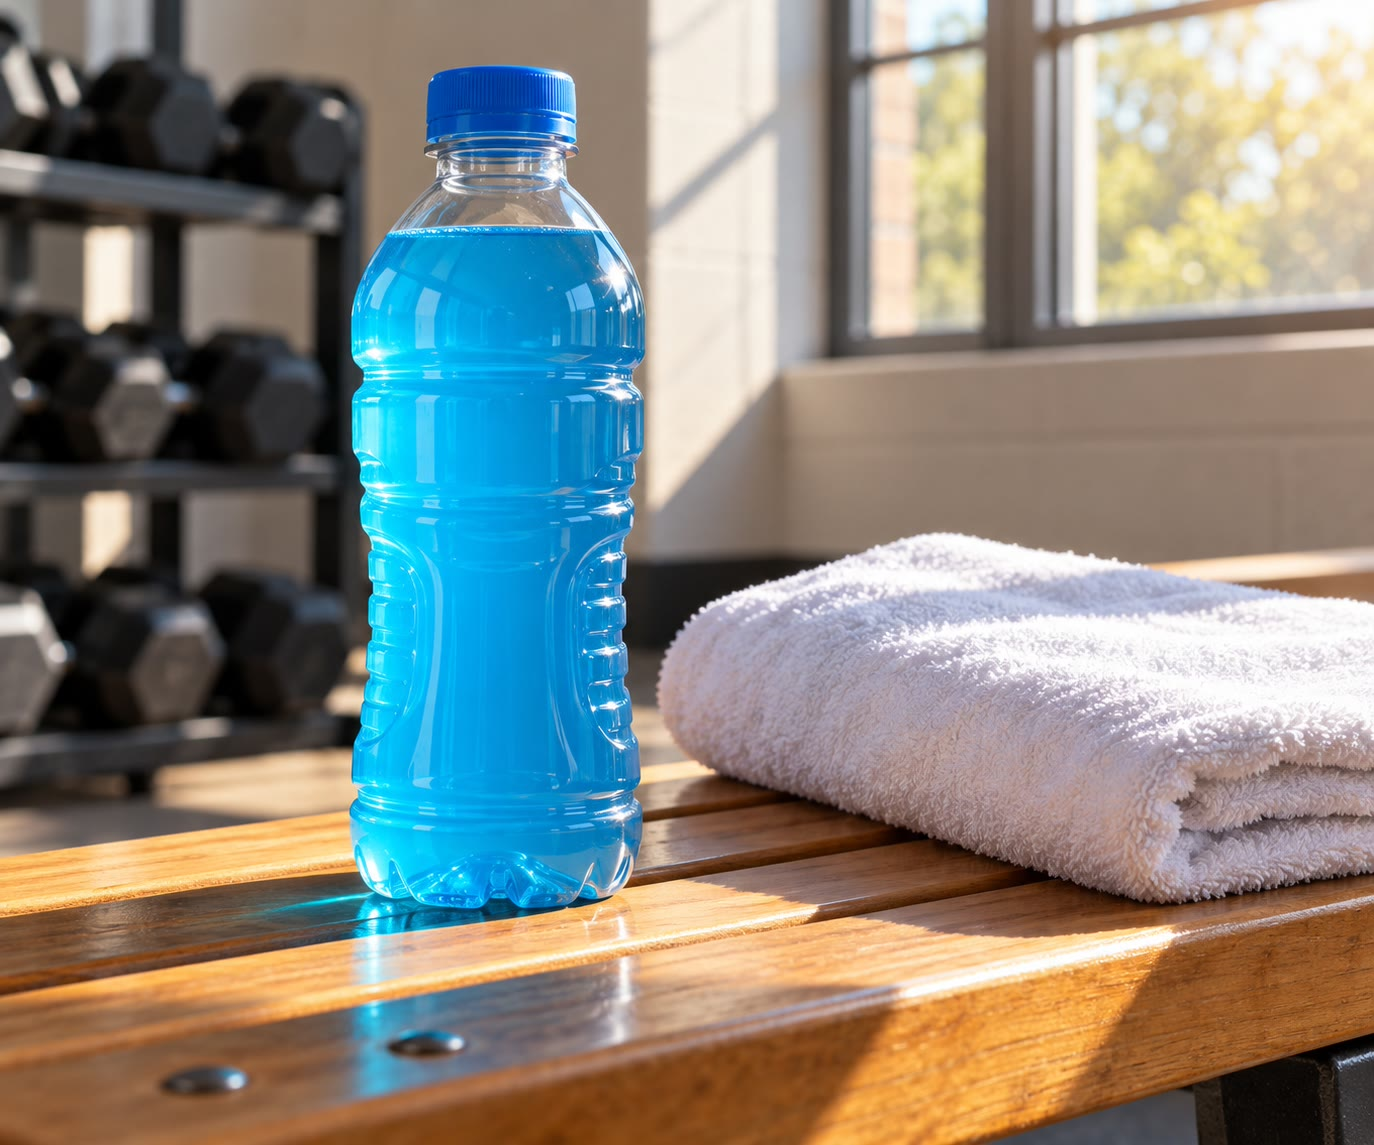
\includegraphics[width=0.5\linewidth]{images/book1/ai/g11-sports-drink.jpg}

{\small एक नीला पेय: उसका रंग प्रति लीटर कुछ मिलीग्राम रंजक से
आता है।}
\end{omfigure}

\section{किसी विलयन का रंग}

श्वेत प्रकाश, जैसे दिन का प्रकाश, इंद्रधनुष के सभी रंगों का \omterm{def:g6:pure-substances-and-mixtures:mixture}{मिश्रण} है। हर रंग एक
तरंगदैर्घ्य के संगत है, बैंगनी के लिए लगभग \qty{400}{nm} से लेकर लाल के लिए
लगभग \qty{750}{nm} तक; तरंगदैर्घ्य क्या है, यह भौतिकी की पुस्तक समझाती है, और
यहाँ वह केवल किसी रंग का एक नाम-पत्र है। रंगीन विलयन अपने से होकर गुज़रने वाले
प्रकाश का कुछ भाग अवशोषित करता है, कुछ रंगों को दूसरों से कहीं अधिक; आँख वे रंग
देखती है जो पार निकल जाते हैं।

\begin{definition}[पूरक रंग]\label{def:g11:absorbance:complementary}
दो रंग \emph{पूरक रंग}\index{पूरक रंग} होते हैं अगर उन्हें मिलाने से श्वेत प्रकाश
बने। रंग-चक्र पर पूरक रंग एक-दूसरे के आमने-सामने
होते हैं।
\end{definition}

\begin{omfigure}
\begin{tikzpicture}[font=\small]
  \foreach \a/\c/\n/\w/\t in {90/red!85!black/लाल/{620--750}/white,
      30/orange/नारंगी/{590--620}/black, -30/yellow!90!orange/पीला/{570--590}/black,
      -90/green!70!black/हरा/{500--570}/white, -150/cyan!50!blue/नीला/{450--500}/white,
      150/violet!80!blue/बैंगनी/{400--450}/white} {
    \fill[\c] (0,0) -- (\a-30:1.8) arc[start angle=\a-30, end angle=\a+30,
      radius=1.8] -- cycle;
    \node[text=\t, font=\small\bfseries] at (\a:1.2) {\n};
    \node[font=\footnotesize, align=center] at (\a:2.45) {\w\\ nm};
  }
  \fill[white] (0,0) circle (0.45);
  \draw[<->, thick, black!70] (90:0.5) -- (-90:0.5);
  \draw[<->, thick, black!70] (30:0.5) -- (-150:0.5);
  \draw[<->, thick, black!70] (-30:0.5) -- (150:0.5);
\end{tikzpicture}

{\small अनुमानित तरंगदैर्घ्यों के साथ एक रंग-चक्र। \omterm{def:g11:absorbance:complementary}{पूरक रंग} एक-दूसरे के
आमने-सामने हैं: लाल और हरा, नारंगी और नीला, पीला और
बैंगनी।}
\end{omfigure}

\begin{proposition}[दिखने वाला रंग]\label{prop:g11:absorbance:colour-seen}
जो विलयन श्वेत प्रकाश के मुख्यतः एक रंग को अवशोषित करता है, वह उसके \omterm{def:g11:absorbance:complementary}{पूरक
रंग} का दिखता है।
\end{proposition}

\begin{proof}
स्वीकृत: पार निकलने वाला प्रकाश श्वेत प्रकाश में से अवशोषित रंग घटाने पर बचा प्रकाश
है, और आँख उस शेष को \omterm{def:g11:absorbance:complementary}{पूरक रंग} के रूप में देखती है।
\end{proof}

\begin{example}[दो खाद्य रंजक]\label{ex:g11:absorbance:dyes}
% ledger: lmax:E133, lmax:E102
स्पोर्ट्स ड्रिंक का नीला रंजक, जिसे ब्रिलियंट ब्लू (E133) कहते हैं,
मुख्यतः नारंगी-लाल प्रकाश अवशोषित करता है, लगभग \qty{629}{nm} पर: वह नीला दिखता है।
पीला रंजक टार्ट्राज़ीन (E102) मुख्यतः बैंगनी-नीला प्रकाश अवशोषित करता है, लगभग
\qty{427}{nm} पर: वह पीला दिखता है। हरे पेय में आम तौर पर दोनों होते हैं।
\end{example}

\section{अवशोषण स्पेक्ट्रम}

\begin{definition}[अवशोषण स्पेक्ट्रम]\label{def:g11:absorbance:spectrum}
किसी विलयन का \emph{अवशोषण स्पेक्ट्रम}\index{अवशोषण स्पेक्ट्रम}
तरंगदैर्घ्य के विरुद्ध उसके द्वारा अवशोषित प्रकाश (उसकी \omterm{def:g11:absorbance:absorbance}{अवशोषकता}, जिसकी परिभाषा अगले
खंड में है) का आलेख है। जिस तरंगदैर्घ्य पर अवशोषण
सबसे अधिक होता है, उसे $\lambda_{\max}$ लिखा जाता है।
\end{definition}

\begin{omfigure}
\begin{tikzpicture}
\begin{axis}[width=0.85\linewidth, height=6cm, xmin=380, xmax=750,
    ymin=0, ymax=0.95, xlabel={तरंगदैर्घ्य $\lambda$ (\si{nm})},
    ylabel={अवशोषकता $A$}, axis lines*=left, ymajorgrids,
    grid style={gray!20}, tick label style={font=\small},
    label style={font=\small}, xtick={400,450,500,550,600,650,700,750},
    ]
  % ledger: lmax:E133, abs:E133, lmax:E102, abs:E102 (band shapes synthetic)
  \addplot[very thick, cyan!60!blue] table[x=lambda, y=E133]
    {figdata/out/grade-11-absorbance-a.dat};
  \addplot[very thick, orange!85!yellow] table[x=lambda, y=E102]
    {figdata/out/grade-11-absorbance-a.dat};
  \node[font=\small, align=left, anchor=west, text=cyan!60!blue!80!black]
    at (axis cs:668,0.62) {नीला रंजक E133,\\ \qty{5.0}{mg/L}};
  \node[font=\small, align=left, anchor=west, text=orange!80!black]
    at (axis cs:470,0.66) {पीला रंजक E102,\\ \qty{15}{mg/L}};
  \addplot[dashed, black!50] coordinates {(629,0) (629,0.82)};
  \addplot[dashed, black!50] coordinates {(427,0) (427,0.795)};
  \node[font=\small, anchor=south] at (axis cs:629,0.83) {\qty{629}{nm}};
  \node[font=\small, anchor=south] at (axis cs:427,0.81) {\qty{427}{nm}};
\end{axis}
\end{tikzpicture}

{\small पानी में दोनों रंजकों के \omterm{def:g11:absorbance:spectrum}{अवशोषण स्पेक्ट्रम}, \qty{1}{cm} मोटे
क्यूवेट में। पट्टों की आकृतियाँ एक सरल मॉडल से बनाई गई हैं; उच्चिष्ठों की
स्थितियाँ और ऊँचाइयाँ दोनों रंजकों के विनिर्देशों से
ली गई हैं।}
\end{omfigure}

\begin{remark}[स्पेक्ट्रम पढ़ना]\label{rem:g11:absorbance:reading}
नीला रंजक \qty{520}{nm} से नीचे लगभग कुछ भी अवशोषित नहीं करता: नीला और बैंगनी
प्रकाश पार निकल जाता है, और विलयन नीला दिखता है। पीला रंजक \qty{520}{nm} से ऊपर
लगभग कुछ भी अवशोषित नहीं करता: हरा, पीला, नारंगी और लाल प्रकाश पार निकल जाता है,
और आँख पीला देखती है। \qty{629}{nm} पर केवल नीला रंजक अवशोषित करता है;
\qty{427}{nm} पर लगभग केवल पीला।
\end{remark}

\section{अवशोषकता और स्पेक्ट्रमप्रकाशमापी}

\begin{definition}[अवशोषकता]\label{def:g11:absorbance:absorbance}
किसी चुने हुए तरंगदैर्घ्य पर किसी विलयन की \emph{अवशोषकता}\index{अवशोषकता} $A$
वह संख्या है जिसे स्पेक्ट्रमप्रकाशमापी दिखाता है, जो मापता है कि विलयन उस
तरंगदैर्घ्य के प्रकाश का कितना भाग अवशोषित करता है। इसका कोई
मात्रक नहीं है; शुद्ध \omterm{def:g6:solutions-and-solubility:solute}{विलायक} के लिए यह शून्य होती है, और विलयन जितना अधिक प्रकाश
अवशोषित करता है, यह उतनी ही बड़ी होती है।
\end{definition}

\begin{omfigure}
\begin{tikzpicture}[font=\small]
  % lamp
  \shade[ball color=yellow!40] (0,0.6) circle (0.32);
  \foreach \a in {0,45,90,135,180,225,270,315} \draw[yellow!60!orange, thick] (\a:0.4) ++(0,0.6) -- ++(\a:0.18);
  \node[anchor=north] at (0,-0.25) {लैंप};
  \draw[black!60, thick] (0.8,0.6) -- (1.75,0.6);
  % prism
  \fill[cyan!10, draw=black!60] (1.75,0.15) -- (2.55,0.15) -- (2.15,1.15) -- cycle;
  \node[anchor=north] at (2.15,-0.25) {प्रिज़्म};
  \foreach \c/\d in {violet/0.35, blue/0.22, green!70!black/0.08, yellow!90!orange/-0.06,
      orange/-0.2, red/-0.34}
    \draw[\c, thick] (2.45,0.6) -- (3.45,{0.6+\d});
  % slit
  \fill[black!70] (3.5,0.92) rectangle (3.6,1.4);
  \fill[black!70] (3.5,-0.2) rectangle (3.6,0.52);
  \node[anchor=north] at (3.55,-0.25) {झिरी};
  \draw[orange, very thick] (3.6,0.6) -- (4.75,0.6);
  % cuvette
  \pic (cv) at (5,0) {cuvette={0.75}{cyan!50!blue!45}};
  \node[anchor=north] at (5,-0.25) {क्यूवेट};
  \draw[orange!60, thick] (5.3,0.6) -- (6.3,0.6);
  % detector and display
  \fill[black!15, draw=black!60] (6.3,0.2) rectangle (6.9,1.0);
  \node[anchor=north] at (6.6,-0.25) {संसूचक};
  \draw[black!60] (6.9,0.6) -- (7.4,0.6);
  \fill[black!80, draw=black] (7.4,0.25) rectangle (9.4,0.95);
  \node[green!70!white, font=\footnotesize\ttfamily] at (8.4,0.6) {A = 0.590};
  \node[anchor=north] at (8.4,-0.25) {प्रदर्शक};
\end{tikzpicture}

{\small स्पेक्ट्रमप्रकाशमापी का सिद्धांत। प्रिज़्म श्वेत प्रकाश को उसके रंगों में
फैला देता है; झिरी केवल एक तरंगदैर्घ्य को आगे जाने देती है, जिसे उपयोगकर्ता चुनता है;
संसूचक क्यूवेट से निकलने वाले प्रकाश की तुलना उसमें प्रवेश करने वाले प्रकाश से
करता है, और प्रदर्शक \omterm{def:g11:absorbance:absorbance}{अवशोषकता} दिखाता है।}
\end{omfigure}

\begin{remark}[यह संख्या कहाँ से आती है]\label{rem:g11:absorbance:log}
उपकरण \omterm{def:g11:absorbance:absorbance}{अवशोषकता} की गणना विलयन में प्रवेश करने और उससे निकलने वाले प्रकाश की
तीव्रताओं से करता है, एक ऐसे गणितीय फलन की मदद से जो विद्यालय के अंतिम वर्ष में
आता है: लघुगणक। विश्वविद्यालय का एक खंड इसका सूत्र देता है; यहाँ \omterm{def:g11:absorbance:absorbance}{अवशोषकता}
बस वह है जो उपकरण पढ़ता है।
\end{remark}

\begin{inthelab}[स्पेक्ट्रमप्रकाशमापी को शून्य पर लाना]
क्यूवेट, \omterm{def:g6:solutions-and-solubility:solute}{विलायक} और स्वयं उपकरण थोड़ा प्रकाश अवशोषित करते हैं।
किसी भी मापन से पहले शुद्ध \omterm{def:g6:solutions-and-solubility:solute}{विलायक} से भरा एक क्यूवेट, यानी
\emph{रिक्त विलयन}, उपकरण में रखा जाता है, और उसे चुने हुए तरंगदैर्घ्य पर
$A = 0$ पढ़ने के लिए समायोजित किया जाता है। इसके बाद का हर पाठ्यांक केवल
\omterm{def:g6:solutions-and-solubility:solute}{विलेय} की \omterm{def:g11:absorbance:absorbance}{अवशोषकता} है। क्यूवेटों को हमेशा उनके खुरदरे फलकों से पकड़ा
जाता है, और पोंछा जाता है: साफ़ फलक पर उँगली का निशान भी प्रकाश
अवशोषित करता है।
\end{inthelab}

\begin{omfigure}
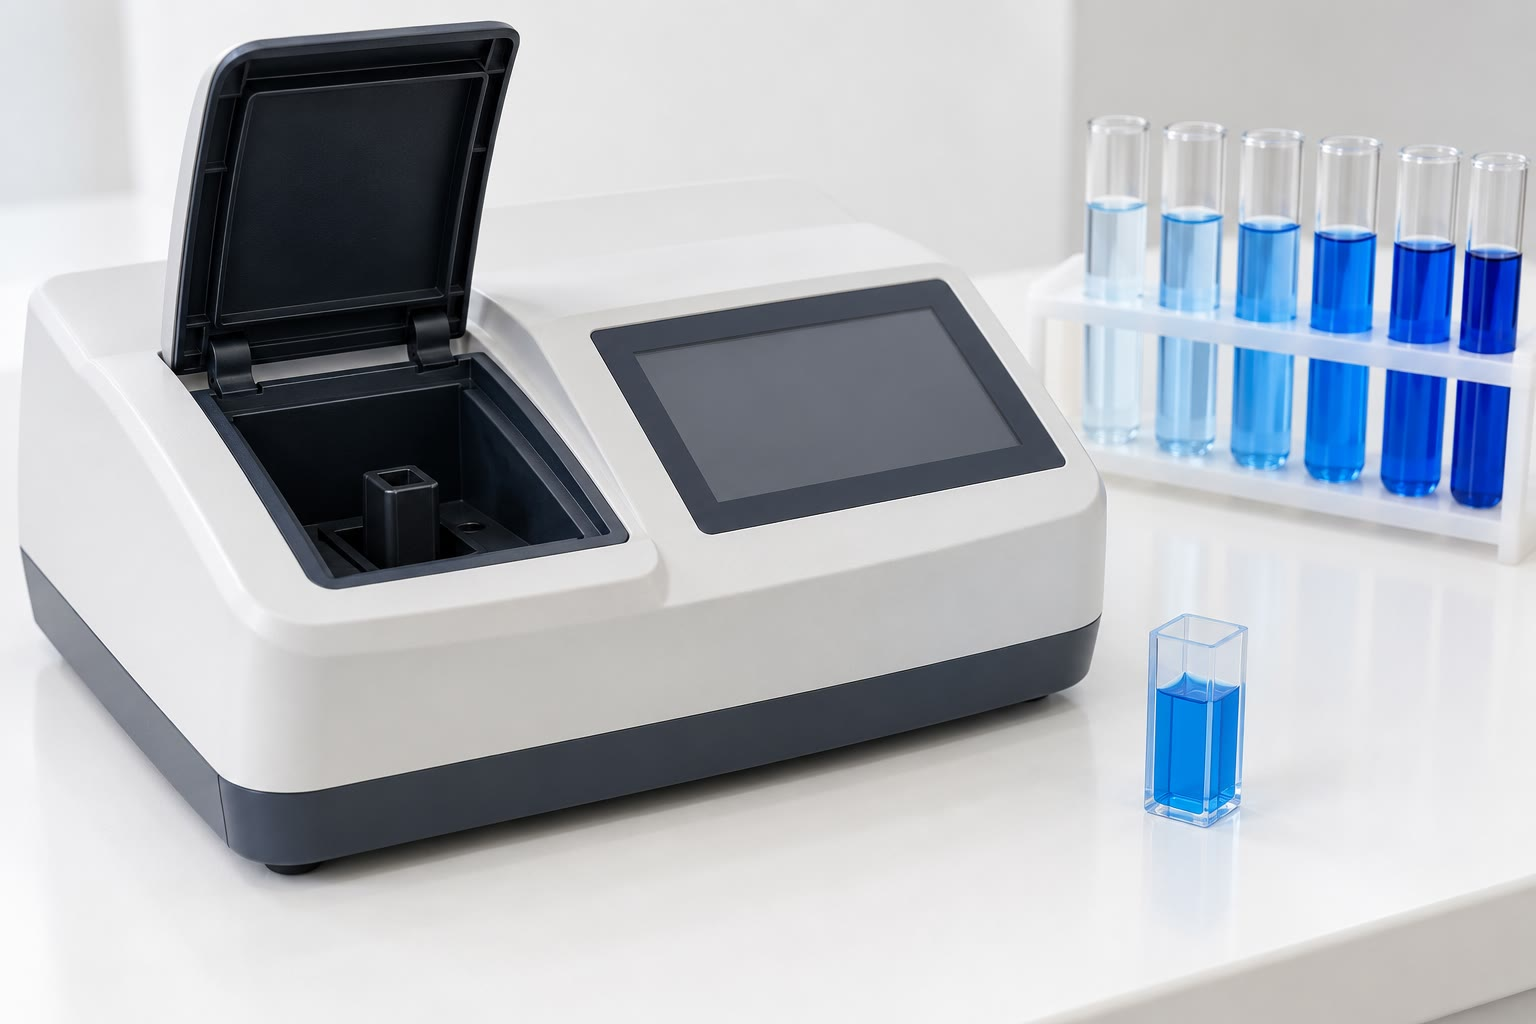
\includegraphics[width=0.5\linewidth]{images/book1/ai/g11-spectrophotometer.jpg}

{\small एक स्पेक्ट्रमप्रकाशमापी और उसके वर्गाकार क्यूवेट।}
\end{omfigure}

\section{बियर--लैम्बर्ट नियम}

\begin{definition}[मोलर अवशोषण गुणांक]\label{def:g11:absorbance:epsilon}
किसी घुली हुई स्पीशीज़ का \emph{मोलर अवशोषण गुणांक}\index{मोलर अवशोषण गुणांक}
$\varepsilon$, किसी दिए गए
तरंगदैर्घ्य पर, मापता है कि उसका एक \omterm{def:g10:the-mole:amount}{मोल} प्रकाश को कितनी तीव्रता से अवशोषित करता है;
यह स्पीशीज़, \omterm{def:g6:solutions-and-solubility:solute}{विलायक} और तरंगदैर्घ्य पर निर्भर करता है, और इसे
\si{L/(mol.cm)} में व्यक्त किया जाता है।
\end{definition}

\begin{proposition}[बियर--लैम्बर्ट नियम]\label{prop:g11:absorbance:beer-lambert}
किसी एक ही अवशोषक स्पीशीज़ के तनु विलयन के लिए, जिसकी \omterm{def:g10:concentration-and-dilution:molar-concentration}{मोलर
सांद्रता} $c$ है, और मोटाई $\ell$ वाले क्यूवेट में, किसी
दिए गए तरंगदैर्घ्य पर \omterm{def:g11:absorbance:absorbance}{अवशोषकता} है
\[
  A = \varepsilon\, \ell\, c .
\]
\omterm{def:g11:absorbance:absorbance}{अवशोषकता} सांद्रता के समानुपाती होती है।
\end{proposition}

\begin{proof}
यहाँ स्वीकृत; इसकी व्युत्पत्ति विश्वविद्यालय के एक खंड में दी गई है।
\end{proof}


\begin{remark}[द्रव्यमान सांद्रता के साथ]\label{rem:g11:absorbance:mass}
% ledger: abs:E133, mw:E133
चूँकि $c = C_m / M$, नियम को $A = a\, \ell\, C_m$ के रूप में भी लिखा जा सकता है,
जहाँ $a = \varepsilon / M$ है, \si{L/(g.cm)} में। खाद्य रंजकों के विनिर्देश
$a$ देते हैं: \qty{629}{nm} पर नीले रंजक E133 के लिए $a =
\qty{164}{L/(g.cm)}$, और उसके \omterm{def:g10:the-mole:molar-mass}{मोलर द्रव्यमान} \qty{792.9}{g/mol} के साथ
$\varepsilon = 164 \times 792.9 = \qty{1.30e5}{L/(mol.cm)}$। उसका केवल
\qty{5.0}{mg/L} वाला विलयन, \qty{1}{cm} क्यूवेट में, पहले से ही
$A = 164 \times 1 \times 0.0050 = 0.82$ पढ़ता है।
\end{remark}

\begin{remark}[केवल तनु विलयन]\label{rem:g11:absorbance:dilute}
समानुपातिकता केवल तनु विलयनों के लिए सही है, व्यवहार में किसी साधारण उपकरण पर लगभग
1 से 1.5 से कम \omterm{def:g11:absorbance:absorbance}{अवशोषकताओं} के लिए। बहुत सांद्र विलयन को मापने से पहले एक ज्ञात
गुणांक से तनु किया जाता है।
\end{remark}

\section{सांद्रता मापना}

\begin{definition}[अंशांकन रेखा]\label{def:g11:absorbance:calibration-line}
\emph{अंशांकन रेखा}\index{अंशांकन रेखा} किसी एक स्पीशीज़ के \omterm{def:g10:concentration-and-dilution:standard}{मानक विलयनों} की
एक श्रृंखला की \omterm{def:g11:absorbance:absorbance}{अवशोषकता} का, एक ही तरंगदैर्घ्य पर और एक ही क्यूवेट में मापी गई,
उनकी सांद्रता के विरुद्ध आलेख है। जब
बियर--लैम्बर्ट नियम लागू होता है, तो यह मूलबिंदु से गुज़रती एक सीधी रेखा होती है।
\end{definition}

\begin{method}[अंशांकन रेखा से सांद्रता मापना]\label{met:g11:absorbance:calibration}
\begin{enumerate}
  \item स्पीशीज़ का \omterm{def:g11:absorbance:spectrum}{अवशोषण स्पेक्ट्रम} रिकॉर्ड कीजिए और तरंगदैर्घ्य
        $\lambda_{\max}$ चुनिए, जहाँ \omterm{def:g11:absorbance:absorbance}{अवशोषकता} सबसे अधिक होती है और तरंगदैर्घ्य
        की छोटी त्रुटि से सबसे कम बदलती है।
  \item रिक्त विलयन से उपकरण को शून्य पर लाइए।
  \item \omterm{def:g10:concentration-and-dilution:dilution}{मूल विलयन} को तनु करके \omterm{def:g10:concentration-and-dilution:standard}{मानक विलयन} तैयार कीजिए और
        उनकी \omterm{def:g11:absorbance:absorbance}{अवशोषकताएँ} मापिए।
  \item सांद्रता के विरुद्ध $A$ आलेखित कीजिए और बिंदुओं के सबसे क़रीब से गुज़रने
        वाली, मूलबिंदु से होकर जाती सीधी रेखा खींचिए।
  \item अज्ञात को मापिए, ज़रूरत हो तो इतना तनु करके कि उसकी \omterm{def:g11:absorbance:absorbance}{अवशोषकता}
        मानकों की \omterm{def:g11:absorbance:absorbance}{अवशोषकताओं} के बीच आए, और उसकी सांद्रता रेखा पर
        पढ़िए (या $A$ को ढाल से भाग दीजिए); \omterm{def:g10:concentration-and-dilution:dilution}{तनुकरण गुणांक} से
        गुणा कीजिए।
\end{enumerate}
\end{method}

\begin{omfigure}
\begin{tikzpicture}
\begin{axis}[width=0.72\linewidth, height=6cm, xmin=0, xmax=5.6,
    ymin=0, ymax=0.95, xlabel={E133 की सांद्रता (\si{mg/L})},
    ylabel={\qty{629}{nm} पर अवशोषकता}, axis lines*=left, ymajorgrids,
    xmajorgrids, grid style={gray!20}, tick label style={font=\small},
    label style={font=\small}]
  % ledger: abs:E133 (points synthetic: exact values + fixed offsets)
  \addplot[only marks, mark=*, mark size=2.2pt, omDef] table[x=C, y=A]
    {figdata/out/grade-11-absorbance-b.dat};
  \addplot[thick, omProp, domain=0:5.5] {0.164*x};
  \addplot[dashed, black!60] coordinates {(0,0.590) (3.6,0.590) (3.6,0)};
  \node[font=\small, anchor=south west] at (axis cs:0.1,0.6) {अज्ञात: $A = 0.590$};
  \node[font=\small, anchor=west] at (axis cs:3.65,0.22) {\qty{3.6}{mg/L}};
\end{axis}
\end{tikzpicture}

{\small नीले रंजक की \omterm{def:g11:absorbance:calibration-line}{अंशांकन रेखा}: पाँच मानक (बिंदु) और
मूलबिंदु से गुज़रती रेखा, जिसका ढाल \qty{0.164}{L/mg} है। $A = 0.590$ पढ़ने
वाले अज्ञात की सांद्रता $0.590 / 0.164 =
\qty{3.6}{mg/L}$ है।}
\end{omfigure}

\begin{example}[पाँच मानक]\label{ex:g11:absorbance:standards}
\qty{100}{mg/L} वाले नीले रंजक के \omterm{def:g10:concentration-and-dilution:dilution}{मूल विलयन} को तनु करके हर मानक का
\qty{100.0}{mL} बनाया जाता है: \qty{2.0}{mg/L} के लिए \omterm{def:g10:concentration-and-dilution:dilution}{तनुकरण
गुणांक} 50 है, इसलिए \omterm{def:g10:concentration-and-dilution:dilution}{मूल विलयन} के \qty{2.0}{mL} को \qty{100.0}{mL} तक पूरा किया जाता है।
1 से \qty{5}{mg/L} तक के पाँच मानक 0.168, 0.325, 0.494,
0.652 और 0.823 पढ़ते हैं: चित्र की रेखा $0.164 \times C$ से कुछ हज़ारवें भाग के
भीतर।
\end{example}

\section{अभ्यास}

\begin{exercise}[$\star$]\label{exo:g11:absorbance:1}
एक विलयन मुख्यतः नारंगी प्रकाश अवशोषित करता है। वह किस रंग का दिखता है? और जो
विलयन मुख्यतः बैंगनी प्रकाश अवशोषित करता है?
\end{exercise}

\begin{exercise}[$\star$]\label{exo:g11:absorbance:2}
रंग-चक्र की मदद से बताइए कि हरा विलयन मुख्यतः कौन-सा रंग अवशोषित करता है, और वह
रंग तरंगदैर्घ्यों का कौन-सा परास घेरता है।
\end{exercise}

\begin{exercise}[$\star$]\label{exo:g11:absorbance:3}
\omterm{def:g11:absorbance:spectrum}{अवशोषण स्पेक्ट्रमों} पर हर रंजक का तरंगदैर्घ्य $\lambda_{\max}$ और वहाँ उसकी
\omterm{def:g11:absorbance:absorbance}{अवशोषकता} पढ़िए।
\end{exercise}

\begin{exercise}[$\star$]\label{exo:g11:absorbance:4}
\qty{2.0}{mg/L} वाला एक रंजक विलयन $A = 0.30$ पढ़ता है। उसी रंजक का
\qty{6.0}{mg/L} वाला विलयन उसी क्यूवेट में, उसी तरंगदैर्घ्य पर, क्या
पढ़ेगा? और \qty{1.0}{mg/L} पर?
\end{exercise}

\begin{exercise}[$\star$]\label{exo:g11:absorbance:5}
स्पेक्ट्रमप्रकाशमापी का रिक्त विलयन क्या है, और उपकरण को उससे शून्य पर क्यों लाया
जाता है?
\end{exercise}

\begin{exercise}[$\star\star$]\label{exo:g11:absorbance:6}
नीले रंजक की \omterm{def:g11:absorbance:calibration-line}{अंशांकन रेखा} की मदद से उस विलयन की सांद्रता ज्ञात कीजिए जो
$A = 0.41$ पढ़ता है।
\end{exercise}

\begin{exercise}[$\star\star$]\label{exo:g11:absorbance:7}
नीले रंजक को मापने के लिए स्पेक्ट्रमप्रकाशमापी को \qty{550}{nm} के बजाय
\qty{629}{nm} पर क्यों रखा जाए? दो कारण बताइए।
\end{exercise}

\begin{exercise}[$\star\star$]\label{exo:g11:absorbance:8}
बिना तनु किया गया एक पेय \qty{629}{nm} पर $A = 2.4$ पढ़ता है, जो भरोसे के लिए
बहुत अधिक है। उसे पाँच गुना तनु किया जाता है और तब वह $A = 0.48$ पढ़ता है। पेय में
नीले रंजक की सांद्रता ज्ञात कीजिए।
\end{exercise}

\begin{exercise}[$\star\star$]\label{exo:g11:absorbance:9}
% ledger: mw:E102, abs:E102
\qty{15.0}{mg/L} वाला टार्ट्राज़ीन का विलयन \qty{1.00}{cm} क्यूवेट में
\qty{427}{nm} पर $A = 0.795$ पढ़ता है। उसकी अवशोषणता $a$
\si{L/(g.cm)} में निकालिए, फिर उसका \omterm{def:g11:absorbance:epsilon}{मोलर अवशोषण गुणांक} (\omterm{def:g10:the-mole:molar-mass}{मोलर द्रव्यमान}
\qty{534.4}{g/mol})।
\end{exercise}

\begin{exercise}[$\star\star$]\label{exo:g11:absorbance:10}
दोनों रंजकों के स्पेक्ट्रम देखिए। किस तरंगदैर्घ्य से ऊपर पीला रंजक लगभग कुछ भी
अवशोषित नहीं करता? पीले रंजक वाले हरे पेय में भी नीले रंजक को
\qty{629}{nm} पर क्यों मापा जा सकता है?
\end{exercise}

\begin{exercise}[$\star\star$]\label{exo:g11:absorbance:11}
उसी विलयन को \qty{1.0}{cm} के बजाय \qty{2.0}{cm} मोटे क्यूवेट में मापा जाता
है। उसकी \omterm{def:g11:absorbance:absorbance}{अवशोषकता} कैसे बदलती है? क्यों?
\end{exercise}

\begin{exercise}[$\star\star\star$]\label{exo:g11:absorbance:12}
नीले रंजक के 5, 10, 20 और \qty{40}{mg/L} वाले मानक 0.82, 1.62,
2.30 और 2.70 पढ़ते हैं। हर एक के लिए $A / C$ निकालिए। आप क्या देखते हैं? \omterm{def:g11:absorbance:calibration-line}{अंशांकन
रेखा} के लिए किन मानकों का उपयोग किया जा सकता है, और $2.5$ पढ़ने वाले अज्ञात के साथ
क्या करना चाहिए?
\end{exercise}

\begin{exercise}[$\star\star\star$]\label{exo:g11:absorbance:13}
एक हरे पेय में नीला रंजक और पीला रंजक हैं। \qty{1.00}{cm} क्यूवेट में वह
\qty{629}{nm} पर $A = 0.574$ और \qty{427}{nm} पर $A = 0.53$
पढ़ता है। \qty{427}{nm} पर नीला रंजक लगभग कुछ भी अवशोषित नहीं करता,
और \qty{629}{nm} पर पीला रंजक कुछ भी अवशोषित नहीं करता। दोनों रंजकों की \omterm{def:g10:concentration-and-dilution:mass-concentration}{द्रव्यमान
सांद्रताएँ} ज्ञात कीजिए ($a = \qty{164}{L/(g.cm)}$ और
$a = \qty{53.0}{L/(g.cm)}$ का उपयोग कीजिए)।
\end{exercise}

\begin{exercise}[$\star\star\star$]\label{exo:g11:absorbance:14}
एक छात्रा रिक्त विलयन भूल जाती है और उपकरण को एक ख़ाली क्यूवेट से शून्य पर लाती
है। तब हर पाठ्यांक \num{0.040} अधिक आता है। अज्ञात
$0.368$ पढ़ता है, और वह इसे वास्तविक \omterm{def:g11:absorbance:calibration-line}{अंशांकन रेखा} के ढाल $0.164$ से भाग देती
है। उसे कौन-सी सांद्रता मिलती है? वास्तविक सांद्रता क्या है? उसकी त्रुटि कितने
प्रतिशत है?
\end{exercise}

\begin{exercise}[$\star\star\star$]\label{exo:g11:absorbance:15}
% ledger: adi:E102
टार्ट्राज़ीन का स्वीकार्य दैनिक अंतर्ग्रहण शरीर के द्रव्यमान के प्रति किलोग्राम
\qty{10}{mg} है। एक पेय में उसका \qty{20}{mg/L} है। पेय का कितना आयतन
\qty{60}{kg} के वयस्क को एक दिन में इस अंतर्ग्रहण तक पहुँचा देगा? क्या
यह एक वास्तविक जोखिम है?
\end{exercise}

\section{समस्या: स्पोर्ट्स ड्रिंक का नीला रंग}


\begin{problem}[{सप्ताहांत समस्या --- किसी बच्चे को नीले स्पोर्ट्स ड्रिंक की कितनी
बोतलें पीनी होंगी ताकि वह उसके रंजक की सुरक्षित दैनिक सीमा तक
पहुँचे?}]
\label{pb:g11:absorbance:1}
% ledger: lmax:E133, abs:E133, mw:E133, adi:E133
एक खाद्य प्रयोगशाला \qty{500}{mL} की बोतलों में बिकने वाले एक स्पोर्ट्स ड्रिंक के नीले
रंजक E133 की जाँच करती है। रंजक के विनिर्देश उसका \omterm{def:g10:the-mole:molar-mass}{मोलर द्रव्यमान},
\qty{792.9}{g/mol}, और उसका स्वीकार्य दैनिक अंतर्ग्रहण देते हैं: शरीर के द्रव्यमान के
प्रति किलोग्राम प्रति दिन \qty{6}{mg}, एक ऐसी मात्रा जिसे जीवन भर हर दिन बिना किसी
उल्लेखनीय जोखिम के खाया जा सकता है।

\medskip
\noindent\textbf{भाग I --- रंग और स्पेक्ट्रम।}
\begin{enumerate}
  \item पेय नीला दिखता है। रंग-चक्र की मदद से बताइए कि वह किस रंग का
        प्रकाश सबसे अधिक अवशोषित करता है?
  \item उसके स्पेक्ट्रम पर रंजक का तरंगदैर्घ्य $\lambda_{\max}$ पढ़िए।
  \item \qty{450}{nm} पर रंजक की \omterm{def:g11:absorbance:absorbance}{अवशोषकता} लगभग शून्य क्यों है?
        क्या यह उसके रंग से मेल खाता है?
  \item मापन किस तरंगदैर्घ्य पर किए जाने चाहिए?
\end{enumerate}

\medskip
\noindent\textbf{भाग II --- \omterm{def:g11:absorbance:calibration-line}{अंशांकन रेखा}।}
\begin{enumerate}[resume]
  \item \qty{50.0}{mg} शुद्ध रंजक घोलकर \qty{500.0}{mL}
        \omterm{def:g10:concentration-and-dilution:dilution}{मूल विलयन} बनाया जाता है। उसकी \omterm{def:g10:concentration-and-dilution:mass-concentration}{द्रव्यमान सांद्रता} \si{mg/L} में निकालिए।
  \item 1.0, 2.0, 3.0, 4.0 और \qty{5.0}{mg/L} के मानक बनाए जाते हैं,
        हर एक \qty{100.0}{mL}। \qty{3.0}{mg/L} वाले मानक के लिए \omterm{def:g10:concentration-and-dilution:dilution}{मूल विलयन} का कितना
        आयतन चाहिए? किस काँच के उपकरण से?
  \item मानक 0.168, 0.325, 0.494, 0.652 और 0.823 पढ़ते हैं। हर एक के लिए
        $A / C$ निकालिए, और दिखाइए कि बिंदु लगभग \qty{0.164}{L/mg} ढाल वाली,
        मूलबिंदु से गुज़रती एक रेखा के क़रीब हैं।
  \item रेखा को मूलबिंदु से क्यों गुज़रना चाहिए?
  \item रंजक की अवशोषणता $a$ \si{L/(g.cm)} में निकालिए (\qty{1.00}{cm} का
        क्यूवेट), फिर उसका \omterm{def:g11:absorbance:epsilon}{मोलर अवशोषण गुणांक}।
\end{enumerate}

\medskip
\noindent\textbf{भाग III --- पेय।}
\begin{enumerate}[resume]
  \item \qty{25.0}{mL} पेय को पानी से \qty{50.0}{mL} तक पूरा किया जाता है।
        \omterm{def:g10:concentration-and-dilution:dilution}{तनुकरण गुणांक} क्या है?
  \item तनु किया गया पेय $A = 0.590$ पढ़ता है। उसमें रंजक की सांद्रता ज्ञात
        कीजिए।
  \item स्वयं पेय में रंजक की सांद्रता निकालिए।
  \item बिना तनु किया पेय क्या पढ़ता? उसे तनु क्यों किया गया?
  \item एक बोतल में रंजक का द्रव्यमान निकालिए।
  \item एक बोतल में रंजक की मात्रा, \omterm{def:g10:the-mole:amount}{मोल} में, निकालिए।
\end{enumerate}

\medskip
\noindent\textbf{भाग IV --- स्वीकार्य दैनिक अंतर्ग्रहण।}
\begin{enumerate}[resume]
  \item \qty{30}{kg} का बच्चा हर दिन रंजक का कितना द्रव्यमान ले
        सकता है?
  \item उस तक पहुँचने के लिए बच्चे को एक दिन में कितनी बोतलें पीनी होंगी?
  \item पेय का यह कितना आयतन है? टिप्पणी कीजिए।
  \item \qty{70}{kg} के वयस्क के लिए यही प्रश्न।
  \item अंतिम उत्तर बताइए: रंजक के स्वीकार्य दैनिक अंतर्ग्रहण तक पहुँचने के लिए
        \qty{30}{kg} के बच्चे को एक दिन में \qty{500}{mL} की कितनी बोतलें पीनी
        होंगी?
\end{enumerate}
\end{problem}
